
\documentclass{beamer}

%\usetheme{Warsaw}
%\usetheme{Antibes}
\usetheme{JuanLesPins}
%\usetheme{Goettingen}

%\usecolortheme{seahorse}
\usecolortheme{dolphin}
%\usecolortheme{rose}
% http://deic.uab.es/~iblanes/beamer_gallery/index_by_color.html
%\usecolortheme{beaver}

%\useoutertheme[]{sidebar}

\setbeamercovered{transparent}

\usepackage[slovak]{babel}
\usepackage[T1]{fontenc}
\usepackage[utf8]{inputenc}
\usepackage{url}

\usepackage{listings}

\lstset{language=C++,basicstyle=\fontsize{8}{9.6}\selectfont,showstringspaces=false,columns=fullflexible,identifierstyle=\ttfamily,keywordstyle=\bfseries,showstringspaces=false,columns=fullflexible}
%\lstset{language=C,basicstyle=\fontsize{10.5}{12.6}\selectfont,identifierstyle=\ttfamily,keywordstyle=\bfseries,showstringspaces=false,columns=fixed}

\def\BibTeX{\textsc{Bib}\kern-.08em\TeX} 

\newcommand{\footcite}[1]{\footnote{\tiny #1}}
\newcommand{\umlet}{.5}
\newcommand{\emp}[1]{\textit{\alert{#1}}}
\newcommand{\kw}[1]{\mbox{\textbf{#1}}}
\newcommand{\id}[1]{\texttt{#1}}
\newcommand{\stl}{\guillemotleft}
\newcommand{\str}{\guillemotright}

\newcommand{\lsti}{\lstinline[basicstyle=\fontsize{10.5}{12.1}\selectfont]}

\newcommand{\ssection}[1]{
	\section{#1}
	\begin{frame}[fragile=singleslide]\frametitle{}
	\Huge #1
	\end{frame}
}

\newcommand{\ssectionn}[1]{
	\section*{#1}
	\begin{frame}[fragile=singleslide]\frametitle{}
	\Huge #1
	\end{frame}
}

\newenvironment{program}{\begin{beamercolorbox}[rounded=true,shadow=true]{block body}\vspace{-4mm}}{\vspace{-2mm}\end{beamercolorbox}}

\setbeamercolor{fvystup}{fg=white,bg=black}
\newenvironment{vystup}{\begin{beamercolorbox}[rounded=true,shadow=true]{fvystup}}{\end{beamercolorbox}}

\newenvironment{poznamka}{\begin{beamercolorbox}[rounded=true,shadow=false]{block body}}{\end{beamercolorbox}}

\setbeamertemplate{footline}[page number]
{
%\insertpagenumber
%\begin{beamercolorbox}{section in head/foot}
%\vskip2pt\insertnavigation{\paperwidth}\vskip2pt
%\end{beamercolorbox}%
}



\author{Tomáš Zenka}
%\url{www.fiit.stuba.sk/~vranic}, \url{vranic@fiit.stuba.sk}}
%{\tiny \url{www.fiit.stuba.sk/~vranic}, \url{vranic@fiit.stuba.sk}}
\institute{
	Ústav informatiky, informačných systémov a softvérového inžinierstva\\
	Fakulta informatiky a informačných technológií\\
	Slovenská technická univerzita v Bratislave}

\subtitle{\vspace{3mm} Metódy inžinierskej práce 2023/2024}

\title{Techniky spracovanie veľkých dát
}

\date{\footnotesize 26. november 2023}




\begin{document}

\begin{frame}[fragile=singleslide]
\titlepage
\end{frame}


\begin{frame}[fragile=singleslide]\frametitle{O čom to je}
V súčasnej ére, kedy sa množstvo dát neustále zväčšuje, stáva sa kľúčovým porozumenie a efektívne spracovanie veľkých objemov informácií. V tejto prezentácii sa ponúka pohľad na nové technológie v oblasti spracovania veľkých dát. Je nevyhnutné pochopiť, aký potenciál majú tieto dáta pre rôzne odvetvia a aké výzvy a príležitosti prinášajú.
\end{frame}


\begin{frame}[fragile=singleslide]\frametitle{Prehľad}
\tableofcontents
\end{frame}


\section{Úvod do sveta veľkých dát}
% príkaz \ssection by vytvoril zvláštný slajd s názvom časti - v krátkych prezentáciách to prekáža, lebo oberá o čas

\begin{frame}[fragile=singleslide]\frametitle{Úvod do sveta veľkých dát}
\begin{itemize}
\item Súbor dát, ktorých veľkosť, komplexnosť a rýchlosť rastu je rapídna
\item Zložité na spracovanie a analýzu
\item Rýchle tempo digitalizácie
\item Za posledné desaťročie sa celkový objem dát zvýšil na 1,8 ZB
\end{itemize}
\end{frame}



\section{Distribuované systémy na spracovanie dát}

\begin{frame}[fragile=singleslide]\frametitle{Distribuované systémy na spracovanie dát}
\begin{itemize}
\item Kľúčový prvok v digitálnom svete
\item Distribuovanie výpočtových úloh na viaceré počítače alebo uzly v sieti
\item Rýchlosť a škálovateľnosť sú najdôležitejšie aspekty
\item Najpoužívanejšie:
	\begin{itemize}
	\item Hadoop: MapReduce
	\item Apache Spark
	\end{itemize}
\end{itemize}
\end{frame}

\begin{frame}[fragile=singleslide]\frametitle{Hadoop: MapReduce}
\begin{itemize}
\item Spoločnosť Google MapReduce
\item V súčastnosti Appache Hadoop:
	\begin{itemize}
	\item Hadoop Kernel
	\item MapReduce
	\item HDFS (Hadoop Distributed File System)
	\end{itemize}
\item Uložiť obrovské množstvo dát
\item Škálovateľnosť
\item Dokáže prežiť zlyhanie významných častí infraštruktúry úložiska
\end{itemize}
\end{frame}


\begin{frame}[fragile=singleslide]\frametitle{Architektúra Apache Hadoop}
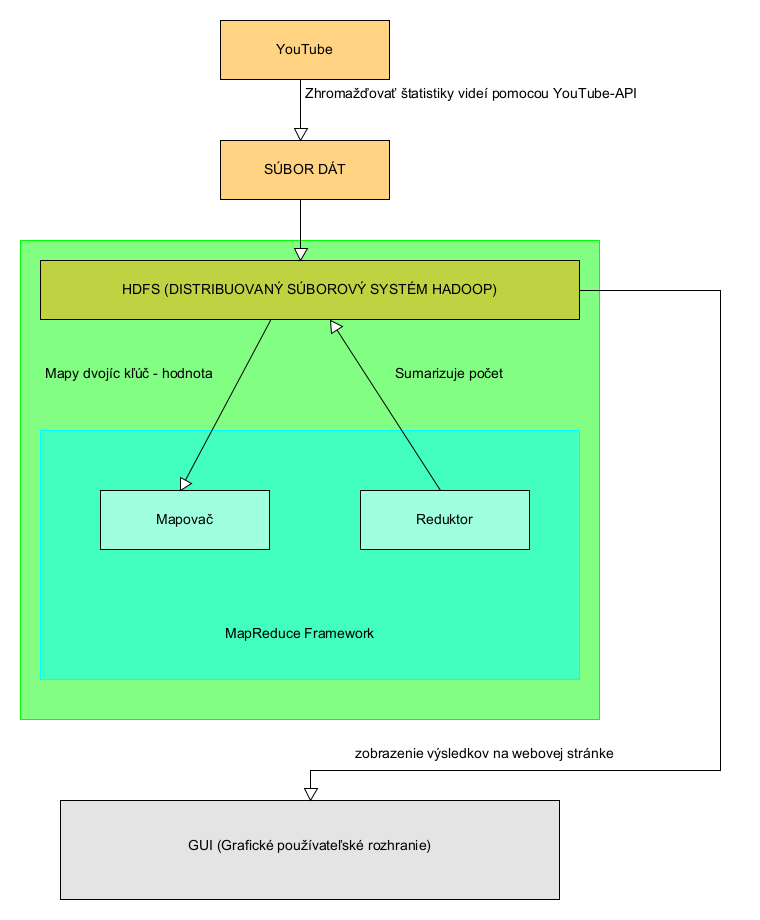
\includegraphics[scale=.23]{HDFS_prelozene.png}
{\tiny Spracované podľa: [6]}
\end{frame}








\begin{frame}[fragile=singleslide]\frametitle{Zvýraznenie syntaxe}
\begin{itemize}
\item Na zvýraznenie syntaxe stačí použiť balík listings so správne nastaveným programovacím jazykom
\begin{lstlisting}
int na_druhu(int i) {
   return i * i;
}

int main() {
   printf("%d", na_druhu(118));
   return 0;
}
\end{lstlisting}

\item Jazyk C++ je ešte zaujímavejší: je multiparadigmový\footcite{\url{J. O. Coplien. Multi-Paradigm Design for C++. Addison-Wesley, 1998.}}
\end{itemize}
\end{frame}


\begin{frame}[fragile=singleslide]\frametitle{Rámiky}
\begin{poznamka}
Text možno uviesť v rámiku
\end{poznamka}

\begin{itemize}
\item Program

\begin{program}
\begin{lstlisting}
void main() {
   printf("%d", na_druhu(118));
}

void na_druhu(int i) {
   return i * i;
}
\end{lstlisting}
\end{program}

\item Výstup
\begin{vystup}
\begin{lstlisting}
13924
\end{lstlisting}
\end{vystup}

\end{itemize}
\end{frame}



\section*{Zhodnotenie a ďalšia práca}
% hviezdička zabezpečí, aby sa táto časť neocitla v prehľade prezentácie - každá prezentácia má zhodnotenie a prehľad by sa tým zbytočne zahlcoval

\begin{frame}[fragile=singleslide]\frametitle{Zhodnotenie a ďalšia práca}
\begin{itemize}
\item Každá prezentácia musí byť nejako uzavretá
\item Ale vždy je čo robiť ďalej\ldots{}
\end{itemize}
\end{frame}

\begin{frame}[allowframebreaks]
\frametitle{Zdroje}
[1] Harshawardhan S Bhosale and Devendra P Gadekar.
A review paper on bigdata and hadoop.
International Journal of Scientic and Research Publications, 4(10):1-7, 2014.

[2] Li Cai and Yangyong Zhu.
The challenges of data quality and data quality assessment in the big data era.
Data science journal, 14:2-2, 2015.

[3] Min Chen, Shiwen Mao, and Yunhao Liu.
Big data: A survey.
MOBILE NETWORKS \& APPLICATIONS, 19(2):171-209, APR 2014.

[4] Bhole Rahul Hiraman, Chapte Viresh M., and Karve Abhijeet C.
A study of apache kafka in big data stream processing.
In 2018 International Conference on Information , Communication, Engineering and Technology (ICICET), pages 1-3, 2018.

[5] Wu Jun and Huang Zhixiong.
Research on in-memory computing model and data analysis.
In 2015 8th International Conference on Intelligent Computation Technology and Automation (ICICTA), pages 726-729, 2015.

[6] PrathyushaRani Merla and Yiheng Liang.
Data analysis using hadoop mapreduce environment.
In 2017 IEEE International Conference on Big Data (Big Data), pages 4783-4785, 2017.

[7] Salman Salloum, Ruslan Dautov, Xiaojun Chen, Patrick Xiaogang Peng, and Joshua Zhexue Huang.
Big data analytics on apache spark.
International Journal of Data Science and Analytics, 1:145-164, 2016.

[8] Eman Shaikh, Iman Mohiuddin, Yasmeen Alufaisan, and Irum Nahvi.
Apache spark: A big data processing engine.
In 2019 2nd IEEE Middle East and North Africa COMMunications Conference (MENACOMM), pages 1-6, 2019.

[9] Chitresh Verma and Rajiv Pandey.
Comparative analysis of gfs and hdfs: Technology and architectural landscape.
In 2018 10th International Conference on Computational Intelligence and Communication Networks (CICN), pages 54-58, 2018.
\end{frame}

\end{document}

\begin{frame}[fragile=singleslide]\frametitle{Slajd len s obrázkom}
\includegraphics[scale=.35]{diagram.pdf}
{\tiny Nejaká poznámka k obrázku, možno zdroj\ldots}
\end{frame}

